% ============================================================= VALIDATION ==
\section{Analysis of validation results}\label{sec:leaderboard}

\subsection{Exact additive identification}
The three row blocks of a submission are disjoint, and each task is scored only on its own rows. Writing
$B=0.35\,\Sstate+0.15\,\Sphys$ for the block that depends on the state rows,
\begin{equation}
  \Stotal = B + 0.20\,\Sodme + 0.15\,\IoU_{\mathrm{onset}} + 0.15\,\IoU_{\mathrm{ongoing}}
  \label{eq:additive}
\end{equation}
holds exactly. Two submissions that differ in one block therefore measure the change of that block exactly, up to
the five-decimal rounding of reported scores ($\pm5\times10^{-6}$ per score, or about $\pm7\times10^{-5}$ in an IoU).
The organizers' baseline table (\cref{tab:baselines}) anchors absolute values: persistence predicts nothing on onset
windows, so its $\Squeue=0.3017$ is half of an ongoing IoU of 0.6034.

Chaining single-block contrasts from that anchor identifies the values in \cref{tab:components}. The chain is
consistent: rebuilding J1 from its identified parts gives 0.84461, exactly its reported score. Two steps (CT1 and CF1)
changed two blocks at once, so the state and ongoing values after them are bounded rather than identified
(\cref{sec:queue-results}). The split of $B$ between $\Sstate$ and $\Sphys$ is not identifiable.

\begin{table}[h]
\centering\small
\caption{Component values identified from validation scores through \cref{eq:additive}. Generated from the submission
record by \code{docs/scripts/make\_figures.py}.}\label{tab:components}
\begin{tabular}{@{}l l r l@{}}
\toprule
Task & Quantity & Value & Identified from \\
\midrule
Demand & $S_{\mathrm{ODME}}$, organizer baseline (TRAIN counts) & 0.8359 & documented \\
 & $S_{\mathrm{ODME}}$, exact NNLS on the split's own counts & 0.9938 & T4-v1 $-$ BASE \\
\addlinespace[2pt]
State & $B$, weekday--slot historical mean (baseline) & 0.2957 & documented \\
 & $B$, time interpolation & 0.4140 & L0 $-$ U2 \\
 & $B$, first residual GBDT (V1) & 0.4226 & P-persq \\
 & $B$, RS1 residual GBDT & 0.4324 & RC2 $-$ RC1 \\
\addlinespace[2pt]
Onset & IoU, persistence (predicts nothing) & $\approx 0$ & by construction \\
 & IoU, first LightGBM, 13 slots incl.\ $T$ (V1) & 0.6393 & V1 $-$ P-noonset \\
 & IoU, legal 12-slot classifier (U1) & 0.6258 & U1 $-$ P-persq \\
 & IoU, train frequency prior (U3) & 0.4497 & U3 $-$ U2 \\
 & IoU, demand-history completion (CS3) & 0.7116 & CS3 $-$ CS2 \\
 & IoU, joint-mask analogue (J1, kept to ES4) & 0.7499 & J1 $-$ U2 \\
\addlinespace[2pt]
Ongoing & IoU, organizer persistence (eligible cells) & 0.6034 & documented \\
 & IoU, first LightGBM, 13 slots incl.\ $T$ (V1) & 0.5922 & P-noonset \\
 & IoU, same, trained on unfiltered windows & 0.6144 & V1-nh $-$ V1 \\
 & IoU, state at slot $T$ (diagnostic only) & 0.7293 & P-slotT $-$ V1 \\
 & IoU, forward-fill of the last legal value (U2) & 0.7381 & U2 $-$ U1 \\
 & IoU, RQ2 analogue decoder (CS1) & 0.7657 & CS1 identity \\
 & IoU, origin analogue (CS2) & 0.7397 & CS2 $-$ CS1 \\
 & $\Delta$IoU, RQ48 quarter-prior decoder & +0.0313 & CF2 $-$ CF1 \\
 & $\Delta$IoU, occupancy classifier RQ59 & -0.0007 & CF3 $-$ CF2 \\
 & $\Delta$IoU, all-month classifier EQ1 & +0.0026 & ES1 $-$ TF3 \\
\bottomrule
\end{tabular}

\end{table}

Three observations follow. The residual state model added 0.127 to $B$ over the historical-mean baseline, more than
any other single change. Onset forecasting moved from zero to 0.750 IoU, worth 0.112 in the composite score. Ongoing
forecasting, which received most of the research effort after the first week, moved from 0.603 to about 0.83, worth
about 0.034.

\subsection{Decomposition of the improvement}
\Cref{tab:steps} decomposes the improvement from the organizer baselines to ES4 into sixteen measured steps. Each
step is the difference between two validation scores; the RS1 and RQ2 steps follow from additivity.

\begin{table}[h]
\centering\small
\caption{Measured steps from the organizer baselines to ES4.}\label{tab:steps}
\begin{tabular}{@{}r l l r r@{}}
\toprule
Step & Change & Rows changed & $\Delta$ score & Cumulative \\
\midrule
0 & Organizer baselines (anchor) & all & & 0.55343 \\\\
1 & Exact split-specific NNLS demand & Demand & +0.03158 & 0.58501 \\
2 & Residual GBDT state reconstruction & State & +0.12691 & 0.71192 \\
3 & Legal onset classifier (U1) & Onset & +0.09387 & 0.80579 \\
4 & Forward-filled ongoing persistence (U2) & Ongoing & +0.02021 & 0.82600 \\
5 & Joint-mask onset analogue (J1) & Onset & +0.01861 & 0.84461 \\
6 & RS1 state model (RC2 $-$ RC1) & State & +0.00974 & 0.85435 \\
7 & RQ2 ongoing analogue decoder (CS1, by additivity) & Ongoing & +0.00414 & 0.85849 \\
8 & S5 speed correction and Q19 features (CT1) & State, ongoing & +0.00039 & 0.85888 \\
9 & S10 factor flow and S12 covariance speed (CT2) & State & +0.00151 & 0.86039 \\
10 & FS1 gate and Q46 first-crossing classifier (CF1) & State, ongoing & +0.00449 & 0.86488 \\
11 & RQ48 quarter-prior decoder (CF2) & Ongoing & +0.00469 & 0.86957 \\
12 & Three-member sample ensemble (TF3) & State & +0.00034 & 0.86991 \\
13 & All-month ongoing classifier (ES1) & Ongoing & +0.00039 & 0.87030 \\
14 & Gap-1 speed recentering (ES2) & State & +0.00039 & 0.87069 \\
15 & Gap-2 speed recentering (ES3) & State & +0.00044 & 0.87113 \\
16 & Gap 3--6 speed recentering (ES4) & State & +0.00074 & 0.87187 \\
\bottomrule
\end{tabular}

\end{table}

\subsection{Transfer of local proxies}\label{sec:transfer}
Seventeen submissions changed the rows of exactly one task relative to an earlier file (\cref{fig:transfer}). Each was
evaluated because a local proxy or a measured rationale favoured it. The contrast between the two panels of the figure
is the most useful methodological result of this work.

\begin{figure}[htbp]
\centering
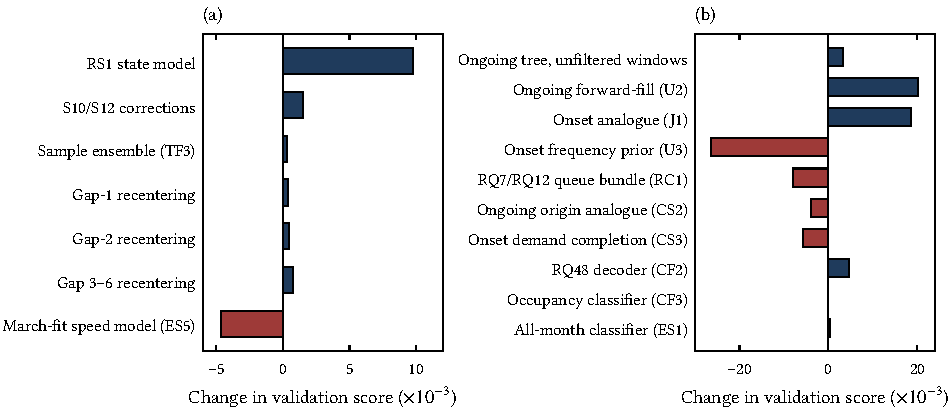
\includegraphics[width=\linewidth]{figures/fig_transfer.pdf}
\caption{Change in validation score of every single-task change: (a) state-only changes, (b) queue-only changes.}\label{fig:transfer}
\end{figure}

\begin{itemize}
  \item \textbf{State changes transferred.} All six state changes selected on held-out training months improved the
        validation score, though by less than the held-out proxies suggested (\cref{sec:state-error}). The single state
        loss, ES5 ($-0.00462$), is the only model fitted and selected on visible cells of the evaluation month itself.
        It lowered visible-cell speed RMSE from 2.545 to 2.006 km/h on every corridor, yet the visible cells were not a
        stand-in for the masked holes.
  \item \textbf{Queue changes did not.} Five of ten queue-only changes lowered the score. CF3's occupancy classifier
        gained 0.0074 to 0.0085 ongoing IoU on visible March proxies and lost 0.0007 on validation; the onset frequency
        prior kept its skill leave-one-month-out on training windows and lost 0.176 onset IoU on validation.
\end{itemize}

Two facts explain the asymmetry. State scores average over millions of cells, so a real improvement is visible; queue
scores average over 80 windows per split. Moreover, the visible-cell and published-window proxies differ in kind from
the hidden targets: visible pseudo-events are noisy observations rather than latent labels, and the published windows
are 80 events from ten days in June.

\subsection{Sampling noise and the private month}
The organizers estimate that queue-window sampling alone moves $\Stotal$ by about 0.0126 (one standard deviation).
The private month has seven incidents against five in the validation month, at different places and times.
Differences of a few thousandths between files are therefore not a reliable forecast of the private ordering, and the
state reconstruction is the most stable part of any composite score.

\subsection{Choice of the final submissions}
Two submissions are scored on the private month. They were chosen for complementary reasons.
\begin{itemize}
  \item \textbf{TF3} is the most defensible artefact: every component was selected on held-out training months under
        pre-registered tests, and the whole file regenerates from the raw release with one command (\cref{sec:repro}).
  \item \textbf{ES4} adds the two later changes that improved the validation score, the all-month ongoing classifier
        and the label-free short-gap recentering, and shares TF3's onset, flow and demand rows exactly.
\end{itemize}
ES5, the only later file, was not selected: it lowered the validation score, and its model was fitted on the
evaluation month.
